En este capítulo se describe la herramienta desarrollada con el propósito de facilitar la aplicación de técnicas de aprendizaje no supervisado en señales bioacústicas.
Se incluyeron diferentes interfaces para la interacción con esta, buscando que el nivel de conocimientos computacionales del usuario no constituya una limitante para el uso de todas las posibilidades que brinda.

En una segunda parte del capítulo, se muestran los experimentos realizados para evaluar los resultados producidos por la herramienta sobre distintas configuraciones de características de audio y conjuntos de datos.

\section{Clusterapp}\label{sec:clusterapp}
\textit{Clusterapp} es la herramienta desarrollada para cumplir los objetivos de este trabajo.
Fue programada empleando el lenguaje de programación \textit{Python}\footnote{https://python.org/} en su versión 3.5;
la decisión se motivó en la flexibilidad del lenguaje y la existencia en este de librerías científicas de reconocido prestigio, adecuadas para su aplicación en este trabajo.

Como se mencionó inicialmente en este capítulo, se tuvo en cuenta al implementar la herramienta que no todos sus usuarios dispondrían de iguales conocimientos computacionales.
Es por ello que se desarrollaron tres variantes para su interacción con la aplicación, cada una adaptada a un perfil de usuario específico.

\subsection{Interfaz web}\label{subsec:interfazWeb}

La interfaz web provee a los usuarios más generales de una variante visual para interactuar con la herramienta.
Los resultados que produce se muestran a través de gráficos y tablas directamente en pantalla, lo que simplifica su análisis.

Para la implementación de esta interfaz se utilizó el framework \textit{Flask}\footnote{http://flask.pocoo.org/}, por su simpleza, velocidad y versatilidad.

En este modo se ofrecen dos vistas diferentes:

\begin{itemize}
    \item \textbf{Análisis de datos}: Vista enfocada al análisis de los patrones existentes en el conjunto de datos y los resultados producidos por diferentes algoritmos de clustering al aplicarse con determinadas configuraciones y características de audio. Puede observarse un ejemplo de esta vista en la figura~\ref{img:dataset-analysis}.
    \item \textbf{Selección de las mejores características}: Esta vista permite determinar el conjunto de características de audio para el que se produce el resultado de mejor evaluación para un algoritmo de clustering dado. Un ejemplo de esta vista aparece en la figura~\ref{img:best-features}.
\end{itemize}

\begin{figure}[!h]
    \centering
    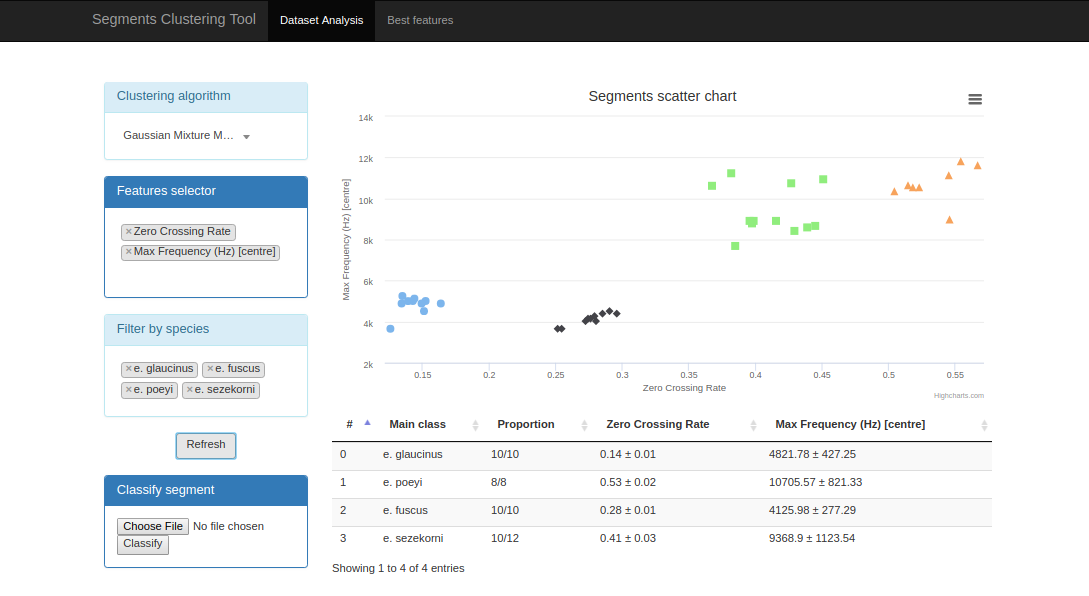
\includegraphics[width=\textwidth]{dataset-analysis.png}
    \caption{Vista de análisis de datos de la interfaz web de la herramienta \textit{Clusterapp}.}
    \label{img:dataset-analysis}
\end{figure}

\begin{figure}[!h]
    \centering
    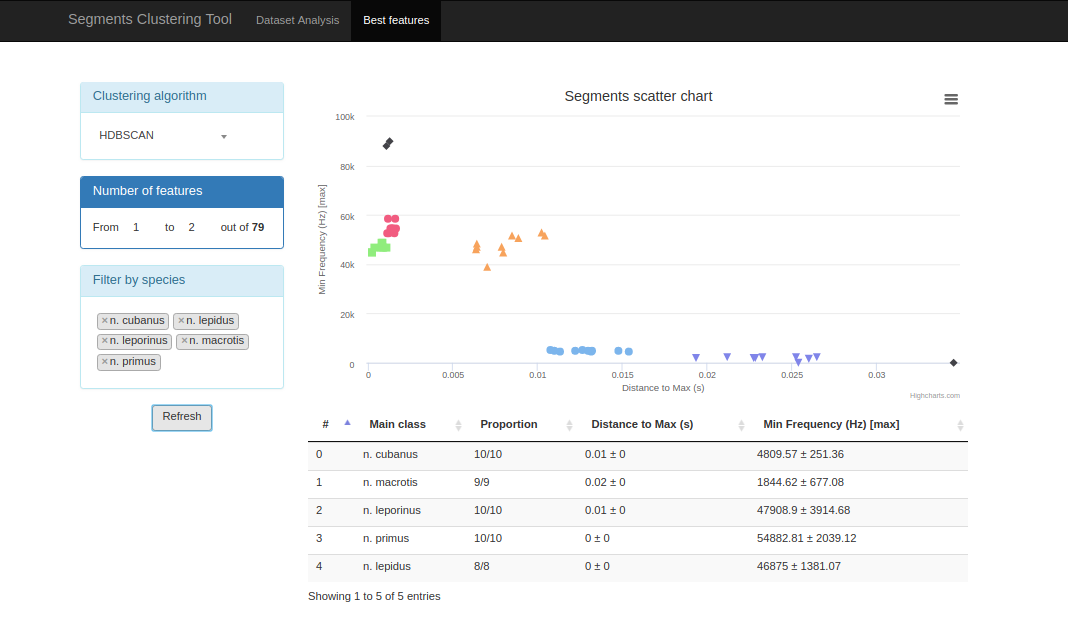
\includegraphics[width=\textwidth]{best-features.png}
    \caption{Vista de selección de las mejores características, de la interfaz web de la herramienta \textit{Clusterapp}.}
    \label{img:best-features}
\end{figure}

Las opciones de configuración en la interfaz web, así como la presentación de los resultados, varían en dependencia de si se dispone o no de información sobre la clasificación real de los segmentos de audio del conjunto de datos sobre el que se realiza el análisis.
Asimismo, en concordancia con dicha información se elige si será supervisado o no, el método para evaluar la calidad de los resultados de los algoritmos;
que es usado en la selección de las características que mejor diferencian los distintos tipos de vocalizaciones presentes en el conjunto de datos.

\subsection{Interfaz de línea de comandos}\label{subsec:CLI}

Mediante esta interfaz, usuarios de mayor experiencia empleando terminales de línea de comandos, pueden interactuar con la herramienta.
Si bien el número de configuraciones que ofrece esta variante es equivalente al de la interfaz web;
a diferencia de en aquella, las configuraciones no son introducidas de forma manual por el usuario, sino que se reciben en un fichero en formato \textit{JSON}.
Ello ofrece mayor rapidez en la ejecución de pruebas con variaciones en la configuración de la herramienta, y que dichas configuraciones puedan ser conservadas en disco para futuras réplicas de los resultados.

Adicionalmente la interfaz de línea de comandos ofrece una ventaja al presentar los resultados en forma más extensiva que su homóloga web.
Los valores obtenidos empleando las distintas medidas de evaluación son directamente mostrados en tablas.
Además, el usuario puede seleccionar si desea que los resultados del clustering con cada variación en la configuración se exporten a ficheros en formato \textit{JSON}, que pueden ser empleados por otras aplicaciones.

\subsection{Librería de Python}\label{subsec:libreríaDePython}

La librería de Python constituye la base sobre la que fueron implementadas las otras dos interfaces.
Se trata de una capa de abstracción entre el código que se encarga de la capa de presentación y el que realiza el cómputo científico.

Esta interfaz ofrece las mismas prestaciones que las ya mencionadas.
Su propósito radica en que puede ser empleada como base sobre la que implementar nuevas interfaces de interacción con el usuario, o para añadir las funcionalidades que provee la herramienta \textit{Clusterapp} directamente dentro de las interfaces de otras aplicaciones.

\section{Conjuntos de datos}\label{sec:datasets}

Para desarrollar los experimentos, se conformaron tres conjuntos de datos con segmentos correspondientes a vocalizaciones de dos \textit{clases} taxonómicas (aves e insectos) y un \textit{orden} taxonómico (murciélagos) respectivamente.
En las tablas~\ref{table:bats-dataset},~\ref{table:birds-dataset} y~\ref{table:insects-dataset} se describen las especies que componen cada uno de estos conjuntos.
Un cuarto conjunto de datos fue constituido a partir de la unión de los anteriores.
De esta forma se comprobó la variación en los resultados en dependencia del grado de parentesco existente entre las especies presentes en los conjuntos de datos.
Todos los segmentos se extrajeron de forma manual a partir de grabaciones de mayor duración.

La diversidad de sonidos que pueden producir los individuos de una misma especie, hace que en la clasificación de los segmentos no baste con recoger simplemente el nombre de la especie de la que proceden.
Por tal razón, se empleó además un identificador para distinguir entre tipos de vocalizaciones diferentes aun cuando estas pudieran provenir de individuos pertenecientes a la misma especie.
De esta forma es posible evaluar mejor los resultados de los algoritmos abordados en este trabajo;
pudiendo distinguirse así entre situaciones en que el algoritmo separó incorrectamente dos clusters de aquellas en que dicha acción tenía sentido por tratarse de tipos de vocalizaciones diferentes.

\section{Resultados}\label{sec:results}

Para la experimentación se emplearon todas las combinaciones de 14 de las características mencionadas en este trabajo:

\begin{multicols}{2}
    \begin{enumerate}
        \item \hyperref[subsec:log-attackTime]{Log-Attack Time}
        \item \hyperref[subsec:audioPower]{Audio Power}
        \item \hyperref[subsec:temporalCentroid]{Temporal Centroid}
        \item \hyperref[subsec:effectiveDuration]{Effective Duration}
        \item \hyperref[subsec:auto-correlation]{Auto-correlation}
        \item \hyperref[subsec:zeroCrossingRate]{Zero Crossing Rate}
        \item \hyperref[itemize:basic-spectral-features]{Frecuencia pico}
        \item \hyperref[itemize:basic-spectral-features]{Frecuencia máxima}
        \item \hyperref[itemize:basic-spectral-features]{Frecuencia mínima}
        \item \hyperref[itemize:basic-spectral-features]{Bandwidth}
        \item \hyperref[subsubsec:spectralCentroid]{Spectral Centroid}
        \item \hyperref[subsubsec:spectrallRollOff]{Spectral Roll-off}
        \item \hyperref[subsec:spectralFlux]{Spectral Flux}
        \item \hyperref[sec:MFCC]{MFCC}
    \end{enumerate}
\end{multicols}

En el caso de las características 2 y 5 se consideró la suma de todos los elementos de dichos vectores.
Para las numeradas entre 7 y 13, se consideró el promedio de los coeficientes correspondientes a las posiciones inicial, final, central, de valor máximo y de máxima amplitud del espectro.
Para los MFCC se empleó el vector obtenido al promediar cada uno de los coeficientes en el tiempo.

Los valores de algunas de las medidas de evaluación, aplicadas a los resultados obtenidos, aparecen resumidos en el Apéndice~\ref{ch:experimentsResults}.

En las figuras~\ref{img:bats},~\ref{img:birds},~\ref{img:insects} y~\ref{img:all} se resume la evaluación de los resultados aplicando el medidor \textit{Adjusted Rand Index};
para tres de estas combinaciones: la conformada por todas las características de la 1 a la 13 (nombradas características \textit{descriptivas}), la que solamente incluye los MFCC, y la que incluye a las 14 características.

\begin{figure}[!h]
    \centering
    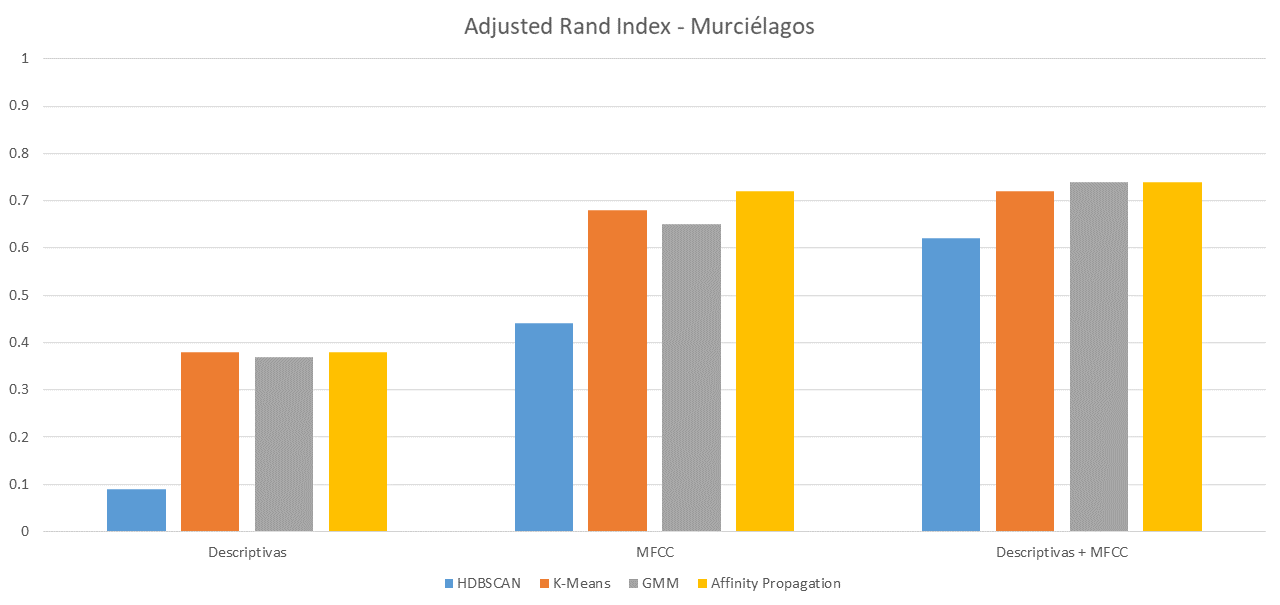
\includegraphics[width=\textwidth]{bats.png}
    \caption{Valores del criterio \textit{Adjusted Rand Index} para el conjunto de datos de murciélagos, en correspondencia con las características y el algoritmo de clustering empleado.}
    \label{img:bats}
\end{figure}

\begin{figure}[!h]
    \centering
    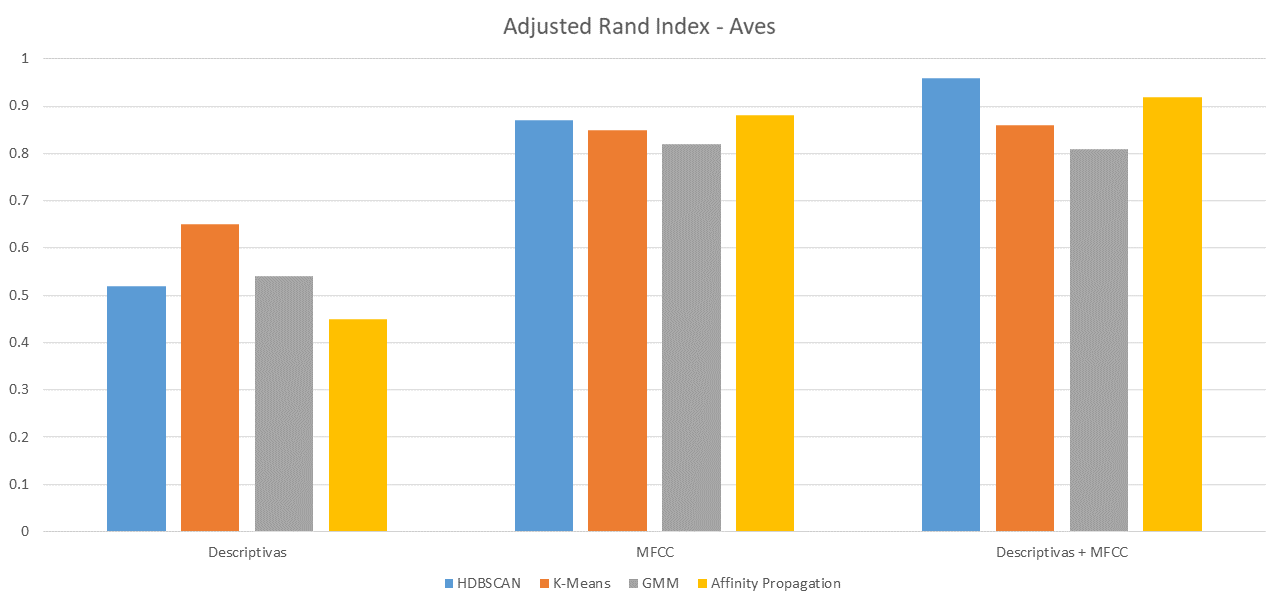
\includegraphics[width=\textwidth]{birds.png}
    \caption{Valores del criterio \textit{Adjusted Rand Index} para el conjunto de datos de aves, en correspondencia con las características y el algoritmo de clustering empleado.}
    \label{img:birds}
\end{figure}

\begin{figure}[!h]
    \centering
    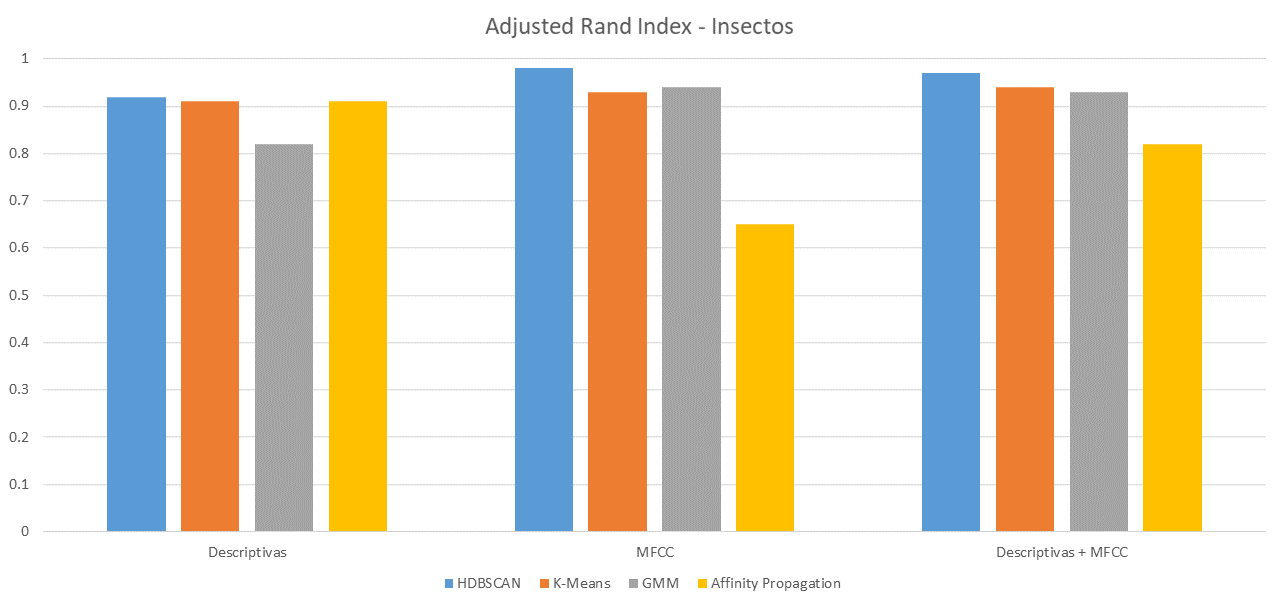
\includegraphics[width=\textwidth]{insects.png}
    \caption{Valores del criterio \textit{Adjusted Rand Index} para el conjunto de datos de insectos, en correspondencia con las características y el algoritmo de clustering empleado.}
    \label{img:insects}
\end{figure}

\begin{figure}[!h]
    \centering
    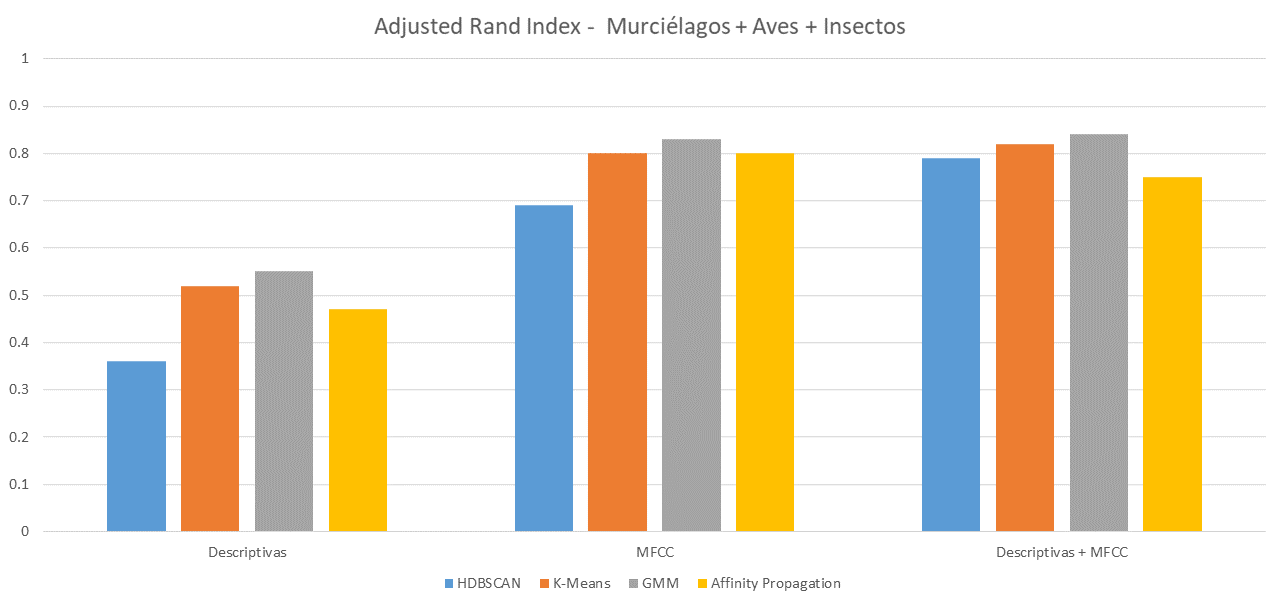
\includegraphics[width=\textwidth]{all.png}
    \caption{Valores del criterio \textit{Adjusted Rand Index} para el conjunto de datos conformado por la unión de los de murciélagos, aves e insectos, en correspondencia con las características y el algoritmo de clustering empleado.}
    \label{img:all}
\end{figure}

Se puede observar que en general los resultados son mucho mejores cuando los MFCC se encuentran presentes en las características utilizadas.
Si bien añadir características adicionales a dicho vector contribuye en la mayoría de los casos a incrementar la calidad del resultado, el valor en que lo hace no es muy significativo.

Puede apreciarse además que la selección del algoritmo no pesa tanto sobre la evaluación del resultado como lo hace la del conjunto de características.

En cuanto a la relación entre el parentesco taxonómico de las especies en el conjunto de datos y la evaluación de los resultados,
los obtenidos en este trabajo muestran mejor comportamiento cuando la diferencia entre las especies se da al nivel de \textit{clase}.
El resultado en el conjunto de los murciélagos soporta la hipótesis de que una relación más estrecha dentro del conjunto de datos deteriora un poco la calidad del resultado.
Lo mismo (aunque al parecer en menor grado) sucede en un conjunto de datos de alta diversidad de organismos.

\nomenclature{JSON}{JavaScript Object Notation}
\nomenclature{ARI}{Índice de Rand Ajustado (por sus siglas en inglés: Adjusted Rand Index)}